\documentclass[runningheads]{llncs}

\usepackage{graphicx}
\usepackage{amsmath}
\usepackage{amssymb}
\usepackage{booktabs}
\usepackage{hyperref}
\usepackage{multirow}

\begin{document}

\title{TransMamba-Cls: Adapting Hybrid Transformer-Mamba Architecture for Text Classification on GLUE Benchmark}
\titlerunning{TransMamba-Cls for Text Classification}

\author{Anonymous Author(s)}
\authorrunning{Anonymous et al.}
\institute{Affiliation anonymized for review}

\maketitle

\begin{abstract}
Recent advances in State Space Models (SSMs), particularly Mamba, have shown competitive performance with Transformers while achieving linear-time complexity. However, hybrid Transformer-SSM architectures have been mainly evaluated on generative and reasoning benchmarks, with limited investigation on discriminative text classification. We present TRANSMAMBA-CLS (where Cls stands for Classification), an adaptation of the TransMamba hybrid architecture for text classification on the GLUE benchmark. Our approach combines a pretrained BERT encoder with a Mamba decoder through a Feature Fusion mechanism employing multi-head cross-attention. We evaluate on two GLUE tasks (SST-2, RTE) across two encoder scales, comparing against BERT baselines and DistilBERT. TransMamba-small achieves the best accuracy among evaluated models on RTE despite having 35\% fewer parameters than DistilBERT, while remaining competitive on SST-2. Our ablation study reveals that the optimal fusion strategy is task-dependent: simpler strategies suffice for short-sequence tasks, while cross-attention provides clear benefits for longer, low-resource tasks.

\keywords{Hybrid Architecture \and Transformer \and Mamba \and Text Classification \and Feature Fusion}
\end{abstract}

% --- SECTION 1 ---
\section{Introduction}
Transformer-based models have become the dominant architecture in Natural Language Processing (NLP), achieving state-of-the-art results across numerous benchmarks [3,13]. However, their quadratic computational complexity $O(n^{2})$ with respect to sequence length poses significant challenges for processing long documents and real-time applications [15,1]. State Space Models (SSMs) [5], particularly Mamba [4], have emerged as a promising alternative with linear-time complexity $O(n)$ through selective scan mechanisms. While Mamba excels at capturing sequential patterns efficiently, it may lack the global contextual understanding provided by self-attention mechanisms in Transformers [12]. 

To bridge this gap, Zhu et al. [17] proposed TransMamba, a hybrid architecture that combines a Transformer encoder with a Mamba decoder through a Feature Fusion mechanism. Their work showed strong performance on reasoning benchmarks (ARC, HellaSwag, PIQA) with a 350M parameter model trained from scratch. However, the applicability of this architecture to text classification tasks remains unexplored. This gap is non-trivial: Mamba's causal selective scan is designed for autoregressive generation, whereas discriminative classification requires bidirectional context understanding. Directly applying generative hybrid models to classification is therefore not straightforward and warrants systematic investigation.

Motivated by this gap, the main contributions of this work are summarized as follows:
\begin{itemize}
    \item We propose TRANSMAMBA-CLS, a hybrid architecture that adapts the TransMamba encoder-decoder framework [17] for discriminative text classification by integrating pretrained BERT encoders with Mamba decoders.
    \item We adapt and evaluate the Feature Fusion mechanism from TransMamba [17], which employs learned projections and multi-head cross-attention to bridge the representation gap between Transformer and SSM modules, for classification tasks on GLUE.
    \item We conduct a systematic empirical evaluation of hybrid Transformer-Mamba architectures on the GLUE text classification benchmark across two encoder scales and two representative tasks to assess the effectiveness of fusion strategies. Notably, TransMamba-small achieves 62.09\% on RTE, outperforming DistilBERT (61.73\%) with 35\% fewer parameters.
\end{itemize}

The remainder of this paper is organized as follows: Section 2 reviews related work, Section 3 describes the proposed methodology, Section 4 presents experimental results, Section 5 provides discussion and analysis, and Section 6 concludes the paper.

% --- SECTION 2 ---
\section{Related Work}

\subsection{Transformer and State Space Models for Text Classification}
Transformer-based pretrained models have dominated text classification benchmarks since the introduction of BERT [3]. The GLUE benchmark [13] serves as the standard evaluation framework, encompassing tasks such as sentiment analysis (SST-2) [11], natural language inference (MNLI) [14], and textual entailment (RTE) [2]. Various BERT variants including DistilBERT [10], ALBERT [6], and RoBERTa [8] have achieved progressively higher scores on these benchmarks. However, these Transformer-based approaches share a common limitation: their $O(n^{2})$ self-attention complexity makes them computationally expensive for long sequences, motivating research into more efficient alternatives.

On the other hand, State Space Models such as S4 [5] and Mamba [4] offer linear-time complexity through selective scan mechanisms, showing competitive results on sequence modeling tasks. However, these SSM-based models have been primarily evaluated on generative language modeling and long-range benchmarks, with fewer studies investigating their effectiveness on standard discriminative classification tasks within the GLUE framework.

\subsection{Hybrid Architectures}
An alternative research direction focuses on combining the strengths of Transformers and SSMs. Zhu et al. [17] proposed TransMamba, which integrates a Transformer encoder with a Mamba decoder through a Feature Fusion mechanism, showing strong performance on reasoning benchmarks. Lieber et al. [7] introduced Jamba, which interleaves Transformer and Mamba layers within a mixture-of-experts framework. These hybrid approaches show promise for combining both global attention and efficient sequential processing. However, existing hybrid architectures have primarily been evaluated on language modeling or reasoning tasks, with limited evaluation on downstream classification benchmarks. This leaves open the question of whether the complementary strengths of Transformer encoders and SSM decoders can benefit discriminative NLP tasks.

\subsection{Positioning of This Work}
Compared with prior studies, the proposed framework differs in several key aspects. First, it adapts the TransMamba hybrid architecture specifically for discriminative text classification rather than language modeling or reasoning. Second, it replaces the custom Transformer encoder with pretrained BERT models, enabling practical deployment with significantly fewer computational resources. Third, it provides one of the few evaluations of a hybrid Transformer-Mamba architecture on discriminative GLUE tasks. Finally, it systematically analyzes the contribution of each fusion component through ablation studies on multiple fusion strategies.

% --- SECTION 3 ---
\section{Methodology}

\subsection{Overview}
The overall architecture of TRANSMAMBA-CLS is illustrated in Fig. 1. The framework follows an encoder-decoder-fusion design, consisting of three main components: (1) a pretrained BERT encoder for extracting global contextual features, (2) a Mamba decoder stack for sequential modeling, and (3) a Feature Fusion module that combines both representations through learned projections and cross-attention.

\begin{figure}[!h]
\centering
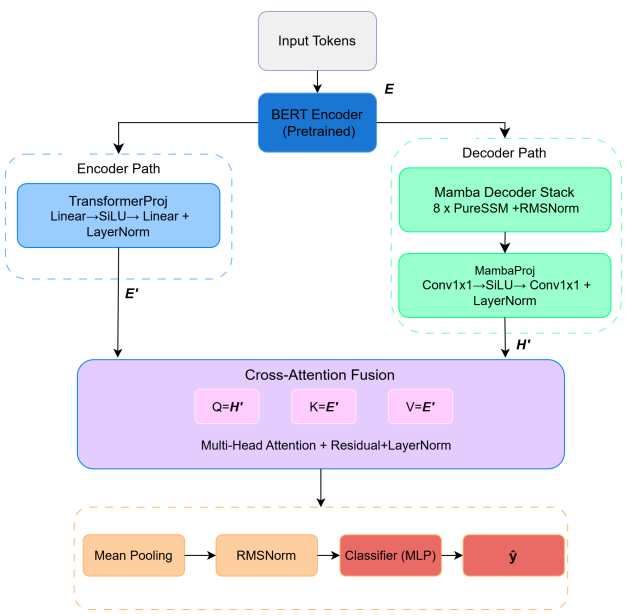
\includegraphics[width=0.75\textwidth]{fig1.png}
\caption{Architecture of TRANSMAMBA-CLS. The pretrained BERT encoder provides global context features $E$, which are processed through two parallel paths: Transformer Proj refines encoder features into $E^{\prime}$, while the Mamba decoder produces sequential features $H$ that are projected into $H^{\prime}$. The cross-attention fusion combines both representations.}
\label{fig:architecture}
\end{figure}

\subsection{Pretrained Transformer Encoder}
Pretrained BERT models [3] are employed as the encoder component. Given an input sequence of tokens $x=(x_{1},x_{2},...,x_{n})$, the encoder produces contextualized representations:
\begin{equation}
E = \text{BERT}(x) \in \mathbb{R}^{n \times d}
\end{equation}
where $d$ is the hidden dimension. Two encoder scales are investigated (Table \ref{tab:encoder_cfg}) to study the relationship between encoder capacity and hybrid model performance.

\begin{table}[h]
\centering
\caption{Encoder configurations used in the experiments.}
\label{tab:encoder_cfg}
\begin{tabular}{lcccc}
\toprule
\textbf{Encoder} & \textbf{Layers} & \textbf{Hidden} & \textbf{Heads} & \textbf{Params} \\
\midrule
BERT-tiny  & 2 & 128 & 2 & 4.4M  \\
BERT-small & 4 & 512 & 8 & 28.8M \\
\bottomrule
\end{tabular}
\end{table}

\subsection{Mamba Decoder Stack}
The decoder consists of $N$ stacked PureSSM layers, a simplified SSM architecture that applies selective state space modeling without gating or MLP sub-layers, with pre-norm using RMSNorm [16]. Each layer applies:
\begin{equation}
y_l = \text{SSM}(\text{RMSNorm}(y_{l-1})) + y_{l-1}
\end{equation}
The Selective State Space Model (SSM) in each layer implements input-dependent discretization and selective scanning:
\begin{equation}
h_{t}=\overline{A}h_{t-1}+\overline{B}x_{t}, \quad y_{t}=Ch_{t}+Dx_{t}
\end{equation}
where $\overline{A}=\exp(\Delta A)$ and $\overline{B}=(\Delta A)^{-1}(\exp(\Delta A)-I)\cdot B$ are the discretized state matrices, and $\Delta$ is the input-dependent step size [4]. In this work, $N=8$ decoder layers are used. The original TransMamba employs 8 encoder and 16 decoder layers (1:2 ratio); here, the decoder depth is fixed at 8 layers across all encoder scales to isolate the effect of encoder capacity on classification performance.

\subsection{Feature Fusion Module}
The core contribution of the TransMamba architecture is the Feature Fusion mechanism [17], which enables the decoder to attend back to encoder representations. Following Zhu et al. [17], the fusion module consists of four steps: (1) the encoder output $E$ is refined through a two-layer linear projection with SiLU activation to produce $E^{\prime}$; (2) the decoder output $H$ is projected through pointwise convolutions to produce $H^{\prime}$; (3) multi-head cross-attention combines $E^{\prime}$ and $H^{\prime}$ and (4) a residual connection followed by mean pooling produces the final classification.

\noindent\textbf{Step 1: Transformer Feature Projection.} The encoder output is refined through a two-layer projection [17]:
\begin{equation}
E^{\prime}=\text{LN}(E+\text{Linear}_{2d\rightarrow d}(\text{SiLU}(\text{Linear}_{d\rightarrow2d}(E))))
\end{equation}

\noindent\textbf{Step 2: Mamba Feature Projection.} The decoder output is projected using pointwise convolutions [17]:
\begin{equation}
H^{\prime}=\text{LN}(H+\text{Conv1x1}_{2d\rightarrow d}(\text{SiLU}(\text{Conv1x1}_{d\rightarrow2d}(H))))
\end{equation}

\noindent\textbf{Step 3: Cross-Attention.} The projected features are combined through multi-head cross-attention [12]:
\begin{equation}
F = \text{CrossAttn}(Q = H^{\prime}, K = E^{\prime}, V = E^{\prime})
\end{equation}

\noindent\textbf{Step 4: Residual Connection.} The fused output with residual connection, mean pooling and classification:
\begin{equation}
O=\text{LN}(H^{\prime}+F), \quad \hat{y}=\text{MLP}(\text{RMSNorm}(\text{MeanPool}(O)))
\end{equation}

\subsection{Training Strategy}
A differential learning rate strategy is adopted: encoder learning rate $\alpha_{e}=2\times10^{-5}$ and decoder/fusion learning rate $\alpha_{d}=5\times10^{-4}$, both with weight decay 0.01. The encoder learning rate follows the standard BERT fine-tuning convention [3] to preserve pretrained representations, while the higher decoder rate is set to accelerate convergence for the randomly initialized Mamba layers, consistent with the training configuration of the original TransMamba [17]. The AdamW optimizer [9] is used with linear warmup (10\% of total steps) followed by cosine decay, and gradient clipping with max norm 1.0. These settings follow the defaults recommended by Loshchilov and Hutter [9].

% --- SECTION 4 ---
\section{Results}

\subsection{Experimental Setup}
The experiments are conducted on two representative tasks from the GLUE benchmark [13] (Table \ref{tab:dataset}), loaded via the Hugging Face datasets library (version 2.16). Tasks are selected to cover diverse aspects of language understanding: data scale (large vs. small), task type (single-sentence vs. sentence-pair), and sequence length (short vs. long).

\begin{table}[h]
\centering
\caption{Dataset statistics for the GLUE tasks used in the evaluation.}
\label{tab:dataset}
\begin{tabular}{lcccc}
\toprule
\textbf{Task} & \textbf{Type} & \textbf{Labels} & \textbf{Train / Dev} & \textbf{Avg Len} \\
\midrule
SST-2 & Sentiment & 2 (pos/neg) & 67,349 / 872 & $\sim$19 \\
RTE & Entailment & 2 (ent/not ent) & 2,490 / 277 & $\sim$60 \\
\bottomrule
\end{tabular}
\end{table}

\begin{itemize}
    \item \textbf{SST-2 (Stanford Sentiment Treebank)} [11]: a binary sentiment classification task on movie reviews. With 67,349 training examples and an average length of $\sim$19 tokens, SST-2 is the most commonly reported GLUE task and serves as the primary benchmark.
    \item \textbf{RTE (Recognizing Textual Entailment)} [2]: a binary entailment task with only 2,490 training examples, making it the smallest dataset in this evaluation. Its premises average $\sim$60 tokens, substantially longer than SST-2, where the Mamba decoder's sequential memory may provide benefits.
\end{itemize}

TRANSMAMBA-CLS is compared against four baselines: (1) BERT-tiny, fine-tuning with a classification head (4.4M params, encoder-only); (2) BERT-small, fine-tuning with a classification head (28.8M params, encoder-only), providing a fair parameter-scale comparison with TransMamba-small; (3) DistilBERT [10], a knowledge-distilled model (66.9M params, encoder-only), representing a competitive SOTA baseline; (4) Pure Mamba, a standalone PureSSM model (4 layers, $d=256$) with word embeddings trained from scratch (9.7M params, decoder-only). The complete training configuration is summarized in Table \ref{tab:hyperparams}.

Input sequences are tokenized using the corresponding BERT WordPiece tokenizer from HuggingFace, with a maximum length of 128 tokens (truncation applied when necessary). The tokenized output, including [CLS] and [SEP] tokens, is passed through the BERT encoder; the full sequence of hidden states is then fed to the Mamba decoder. Accuracy on the development set is reported as the primary metric. The evaluation on larger NLI tasks (e.g., MNLI) is left for future work due to computational constraints. Source code will be released upon acceptance.

\begin{table}[h]
\centering
\caption{Training hyperparameters and environment.}
\label{tab:hyperparams}
\begin{tabular}{ll}
\toprule
\textbf{Hyperparameter} & \textbf{Value} \\
\midrule
Encoder LR & $2\times10^{-5}$ \\
Decoder/Fusion LR & $5\times10^{-4}$ \\
Optimizer & AdamW (weight decay 0.01) \\
Scheduler & Cosine decay with 10\% warmup \\
Batch size & 32 \\
Max sequence length & 128 \\
Epochs (SST-2/RTE) & 5 / 15 \\
Gradient clipping & max norm 1.0 \\
Mamba decoder layers & 8 \\
Mamba $d_{model}$ & matches encoder d \\
Random seed & 42 \\
GPU / Framework & NVIDIA RTX 4090 / RTX 3060 / T4, PyTorch 2.1+, Transformers 4.37 \\
\bottomrule
\end{tabular}
\end{table}

\subsection{Results on GLUE Tasks}
Table \ref{tab:main_results} presents the main comparison results. All TransMamba models use an 8-layer Mamba decoder; the best-performing fusion strategy is selected for each model scale based on the ablation results in Table \ref{tab:ablation}. TransMamba-small uses Cross-Attention without the additional learned projections, which achieved the best overall performance across tasks.

TRANSMAMBA-CLS outperforms the BERT-tiny and Pure Mamba baselines across both tasks. Notably, TransMamba-small achieves the highest accuracy on RTE (62.09\%), outperforming not only BERT-small (61.37\%) at the same encoder scale but also DistilBERT (61.73\%) despite having 35\% fewer parameters (43.6M vs. 66.9M). BERT-base (110M params) is excluded from the direct comparison as it is 2.5x larger than our largest model (43.6M), placing it outside the parameter range targeted by this study. For reference, Devlin et al. [3] report 93.5\% on SST-2 and 66.4\% on RTE with BERT-base.

This indicates that the Mamba decoder provides a complementary advantage for low-resource, longer-sequence tasks that cannot be replicated by simply scaling up encoder-only models. On SST-2, DistilBERT achieves 91.63\%, outperforming TransMamba-small (87.73\%), which suggests that for large-data, short-sequence sentiment classification, pretrained encoder-only models remain highly competitive.

\begin{table}[h]
\centering
\caption{Main results on GLUE development sets. Accuracy (\%) is reported. Training time (minutes) is measured on SST-2. The best result per column is in bold.}
\label{tab:main_results}
\begin{tabular}{lcccc}
\toprule
\textbf{Model} & \textbf{SST-2} & \textbf{RTE} & \textbf{Params} & \textbf{Time (min)} \\
\midrule
\textit{Baselines} & & & & \\
BERT-tiny (encoder-only) & 81.08 & 55.60 & 4.4M & 2.3 \\
BERT-small (encoder-only) & \textbf{88.76} & 61.37 & 28.8M & 19.9 \\
DistilBERT (encoder-only) & 91.63 & 61.73 & 66.9M & 58.6 \\
Pure Mamba (decoder-only) & 82.80 & 53.07 & 9.7M & 65.6 \\
\midrule
\textit{TransMamba-Cls (8L decoder)} & & & & \\
TransMamba-Cls-tiny & 83.49 & 57.04 & 5.5M & 134.1 \\
TransMamba-Cls-small & 87.73 & \textbf{62.09} & 43.6M & 139.1 \\
TransMamba-Cls-small (frozen) & 84.17 & 56.32 & 17.0M & 136.7 \\
\midrule
\textit{Encoder Scaling ($\Delta$: tiny $\rightarrow$ small)} & & & & \\
$\Delta$ TransMamba-Cls & +4.24 & +5.05 & - & - \\
\bottomrule
\end{tabular}
\end{table}

\noindent \textbf{Training Efficiency.} Pure Mamba's longer training time (65.6 min vs. 19.9 min for BERT-small despite fewer parameters) is due to the sequential nature of the PureSSM implementation in PyTorch, which cannot leverage the parallelized operations available in optimized Transformer libraries.

\noindent \textbf{Encoder Scaling.} Increasing the encoder from BERT-tiny (2L, 128d) to BERT-small (4L, 512d) yields consistent gains: +4.24\% on SST-2 and +5.05\% on RTE. This confirms that richer encoder representations benefit the downstream fusion mechanism.

\noindent \textbf{Frozen Encoder.} Freezing the BERT-small encoder (training only the Mamba decoder and fusion module) achieves 84.17\% on SST-2, slightly below the fine-tuned variant but still above both baselines. On RTE, freezing degrades performance to 56.32\%, suggesting that encoder fine-tuning is more critical for low-resource tasks.

\subsection{Ablation Study}
To quantify the contribution of each fusion component, four fusion strategies are evaluated while keeping the encoder (BERT-small) and decoder (8 layers) fixed (Table \ref{tab:ablation}).

\begin{table}[h]
\centering
\caption{Ablation study on fusion strategies using BERT-small encoder and 8-layer Mamba decoder. $^{*}$Evaluated with a frozen encoder due to computational constraints.}
\label{tab:ablation}
\begin{tabular}{llccc}
\toprule
\textbf{Fusion Type} & \textbf{Description} & \textbf{Params} & \textbf{SST-2} & \textbf{RTE} \\
\midrule
None & Only Mamba output & 42.6M & 87.16 & 60.29 \\
Additive & $\text{LN}(H+E)$ & 42.6M & \textbf{87.73} & 58.48 \\
Cross-Attn (Ours) & $\text{CrossAttn}(H,E,E)$ & 43.6M & \textbf{87.73} & \textbf{62.09} \\
Cross-Attn + Proj$^{*}$ & $\text{CrossAttn}(H^{\prime}, E^{\prime}, E^{\prime})$ & 17.0M & 84.17 & 56.32 \\
\bottomrule
\end{tabular}
\end{table}

The ablation reveals several notable patterns. First, the Additive and Cross-Attention fusion strategies achieve the highest accuracy on SST-2 (87.73\%), outperforming the no-fusion baseline. This suggests that for short-sequence sentiment classification with abundant data, both simple addition and attention mechanisms effectively combine the representations.

Second, on RTE (longer sequences, low-resource), Cross-Attention achieves the best performance (62.09%), outperforming the no-fusion baseline by +1.80\% and the Additive fusion by +3.61\%. The attention mechanism allows the model to selectively integrate encoder and decoder representations, which is highly beneficial when sequences are longer and data is scarce.

Third, we evaluate the full projection-based cross-attention (as described in Sec. 3). Due to computational constraints, this variant was trained with a frozen encoder (17.0M trainable parameters). It achieves 84.17\% on SST-2 and 56.32\% on RTE. This lower performance relative to the simple cross-attention demonstrates that end-to-end encoder fine-tuning is far more critical for classification datasets than adding projection parameters to the fusion module.

% --- SECTION 5 ---
\section{Discussion}

\noindent \textbf{Pretrained vs. Custom Encoder.} Unlike the original TransMamba, which trains a custom Transformer encoder from scratch (350M parameters), this work leverages pretrained BERT encoders. This choice is motivated by practical resource constraints (the proposed model is 10-70x smaller), reproducibility through standard Hugging Face checkpoints, and the research focus on fusion effectiveness rather than encoder architecture.

\noindent \textbf{Task-Dependent Fusion Effectiveness.} The ablation study reveals that the optimal fusion strategy is task-dependent. For SST-2 (short sequences, large data), simpler fusions such as None and Additive perform comparably to cross-attention. For RTE (longer sequences, limited data), cross-attention provides a clear advantage (+1.80\% over no fusion). The full projection variant (trained with a frozen encoder) scores lower on both tasks, confirming that encoder fine-tuning matters more than fusion complexity for these datasets.

\begin{figure}[!h]
\centering
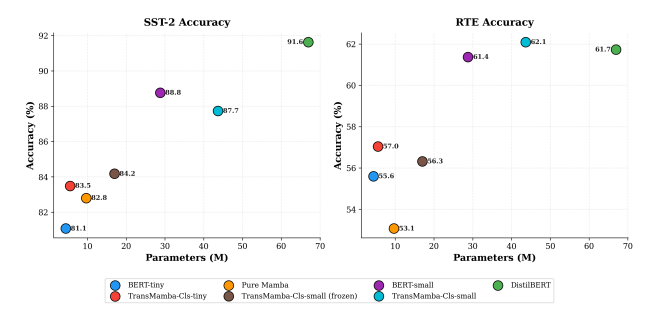
\includegraphics[width=1.0\textwidth]{fig2.png}
\caption{Accuracy vs. number of parameters trade-off on SST-2 (left) and RTE (right). Each circle represents a model; colors distinguish different architectures. On RTE, TransMamba-Cls-small achieves the highest accuracy despite having fewer parameters than DistilBERT.}
\label{fig:tradeoff}
\end{figure}

\noindent \textbf{Frozen Encoder Analysis.} Freezing the BERT-small encoder degrades SST-2 accuracy only slightly (87.73\% $\rightarrow$ 84.17\%) but substantially hurts RTE (62.09\% $\rightarrow$ 56.32factory), suggesting that low-resource tasks benefit more from task-specific encoder adaptation.

\noindent \textbf{Limitations.} The evaluation is limited to two GLUE tasks and sequences of length $<128$ tokens, where the linear-time advantage of Mamba is less pronounced. Evaluation on larger tasks such as MNLI is left for future work. The PureSSM implementation in PyTorch also does not leverage hardware-aware CUDA kernels [4], resulting in slower training compared to optimized alternatives.

% --- SECTION 6 ---
\section{Conclusion}
We presented TRANSMAMBA-CLS, a hybrid Transformer-Mamba architecture adapted for text classification on the GLUE benchmark. By combining pretrained BERT encoders with Mamba decoders through cross-attention fusion, our model achieves the best accuracy among evaluated models on RTE (62.09\%), outperforming both BERT-small (61.37\%) and DistilBERT (61.73\%) despite having significantly fewer parameters. This indicates that the Mamba decoder provides complementary sequential modeling benefits that cannot be achieved by simply scaling encoder-only models.

Our ablation study yields a key insight: the optimal fusion strategy is task-dependent. Simpler strategies such as None and Additive suffice for large-data, short-sequence tasks (SST-2), while cross-attention provides meaningful gains for low-resource tasks with longer sequences (RTE). Moreover, end-to-end encoder fine-tuning proved more important than fusion complexity: the full projection variant with a frozen encoder underperformed the simpler cross-attention with a fine-tuned encoder on both tasks. The observed effectiveness on low-resource tasks suggests potential applicability to domain adaptation scenarios where labeled data is scarce, though this remains to be validated in future work.

Future work includes: (1) evaluation on larger GLUE tasks (e.g., MNLI) and long-document classification where the linear-time advantage of Mamba is more pronounced, (2) exploration of bidirectional Mamba variants (BiMamba) as the decoder, and (3) integration of hardware-optimized Mamba CUDA kernels for improved training efficiency.

% --- REFERENCES ---
\begin{thebibliography}{17}

\bibitem{1} Beltagy, I., Peters, M.E., Cohan, A.: Longformer: The long-document transformer. arXiv preprint arXiv:2004.05150 (2020)

\bibitem{2} Dagan, I., Glickman, O., Magnini, B.: The PASCAL recognising textual entailment challenge. In: Machine Learning Challenges. Evaluating Predictive Uncertainty, Visual Object Classification, and Recognising Textual Entailment, pp. 177–190. Springer (2006)

\bibitem{3} Devlin, J., Chang, M.W., Lee, K., Toutanova, K.: BERT: Pre-training of deep bidirectional transformers for language understanding. In: Proceedings of the 2019 Conference of the North American Chapter of the Association for Computational Linguistics (NAACL-HLT). pp. 4171–4186 (2019)

\bibitem{4} Gu, A., Dao, T.: Mamba: Linear-time sequence modeling with selective state spaces. arXiv preprint arXiv:2312.00752 (2023)

\bibitem{5} Gu, A., Goel, K., Ré, C.: Efficiently modeling long sequences with structured state spaces. In: Proceedings of the International Conference on Learning Representations (ICLR) (2022)

\bibitem{6} Lan, Z., Chen, M., Goodman, S., Gimpel, K., Sharma, P., Soricut, R.: ALBERT: A lite BERT for self-supervised learning of language representations. In: Proceedings of the International Conference on Learning Representations (ICLR) (2020)

\bibitem{7} Lieber, O., Lenz, B., Bata, H., Cohen, G., Osin, J., Dalmedigos, I., Safahi, E., Meirom, S., Belinkov, Y., Shalev-Shwartz, S., Shoham, Y.: Jamba: A hybrid Transformer-Mamba language model. arXiv preprint arXiv:2403.19887 (2024)

\bibitem{8} Liu, Y., Ott, M., Goyal, N., Du, J., Joshi, M., Chen, D., Levy, O., Lewis, M., Zettlemoyer, L., Stoyanov, V.: RoBERTa: A robustly optimized BERT pretraining approach. arXiv preprint arXiv:1907.11692 (2019)

\bibitem{9} Loshchilov, I., Hutter, F.: Decoupled weight decay regularization. In: Proceedings of the International Conference on Learning Representations (ICLR) (2019)

\bibitem{10} Sanh, V., Debut, L., Chaumond, J., Wolf, T.: DistilBERT, a distilled version of BERT: smaller, faster, cheaper and lighter. arXiv preprint arXiv:1910.01108 (2019)

\bibitem{11} Socher, R., Perelygin, A., Wu, J., Chuang, J., Manning, C.D., Ng, A.Y., Potts, C.: Recursive deep models for semantic compositionality over a sentiment treebank. In: Proceedings of the 2013 Conference on Empirical Methods in Natural Language Processing (EMNLP). pp. 1631–1642 (2013)

\bibitem{12} Vaswani, A., Shazeer, N., Parmar, N., Uszkoreit, J., Jones, L., Gomez, A.N., Kaiser, Ł., Polosukhin, I.: Attention is all you need. Advances in Neural Information Processing Systems 30 (2017)

\bibitem{13} Wang, A., Singh, A., Michael, J., Hill, F., Levy, O., Bowman, S.R.: GLUE: A multi task benchmark and analysis platform for natural language understanding. In: Proceedings of the International Conference on Learning Representations (ICLR) (2019)

\bibitem{14} Williams, A., Nangia, N., Bowman, S.R.: A broad-coverage challenge corpus for sentence understanding through inference. In: Proceedings of the 2018 Conference of the North American Chapter of the Association for Computational Linguistics (NAACL-HLT). pp. 1112–1122 (2018)

\bibitem{15} Zaheer, M., Guruganesh, G., Dubey, K.A., Ainslie, J., Alberti, C., Ontanon, S., Pham, P., Ravula, A., Wang, Q., Yang, L., Ahmed, A.: Big Bird: Transformers for longer sequences. In: Advances in Neural Information Processing Systems (NeurIPS) (2020)

\bibitem{16} Zhang, B., Sennrich, R.: Root mean square layer normalization. In: Advances in Neural Information Processing Systems (NeurIPS). vol. 32 (2019)

\bibitem{17} Zhu, Y., Wang, Y., Wang, X., Wang, Z., Liu, Z.: TransMamba: Flexibly switching between transformer and mamba. arXiv preprint arXiv:2501.07948 (2025)

\end{thebibliography}

\end{document}